\comment{
https://www.iaria.org/conferences2016/filesICSNC16/Softnet2016_Tutorial_Fog-MEC-Cloudlets-E.Borcoci-v1.1.pdf

this paper has it nailed down with terms https://arxiv.org/pdf/1812.00591.pdf 
}

\subsection{Terms and Definitions} \label{sec:definitions}
The IoT and edge landscape is hard to understand, especially because terms are loosely and inconsistently defined. Similar is true for the cloud but it uses less diverse technologies and is thus less confusing. This section will explain the network topology, key terms and their concepts as the foundation for the following report.\\
\vspace{0.5mm} \ \\
\textbf{\textit{Network Topology}}\\
\Cref{fig:networkTopology3Layer} shows the network topology used in this report. 
% The focus will be on the management and security of the device edge as well as its interaction with the IoT devices themselves. 
\begin{figure}[H]
    \centering
    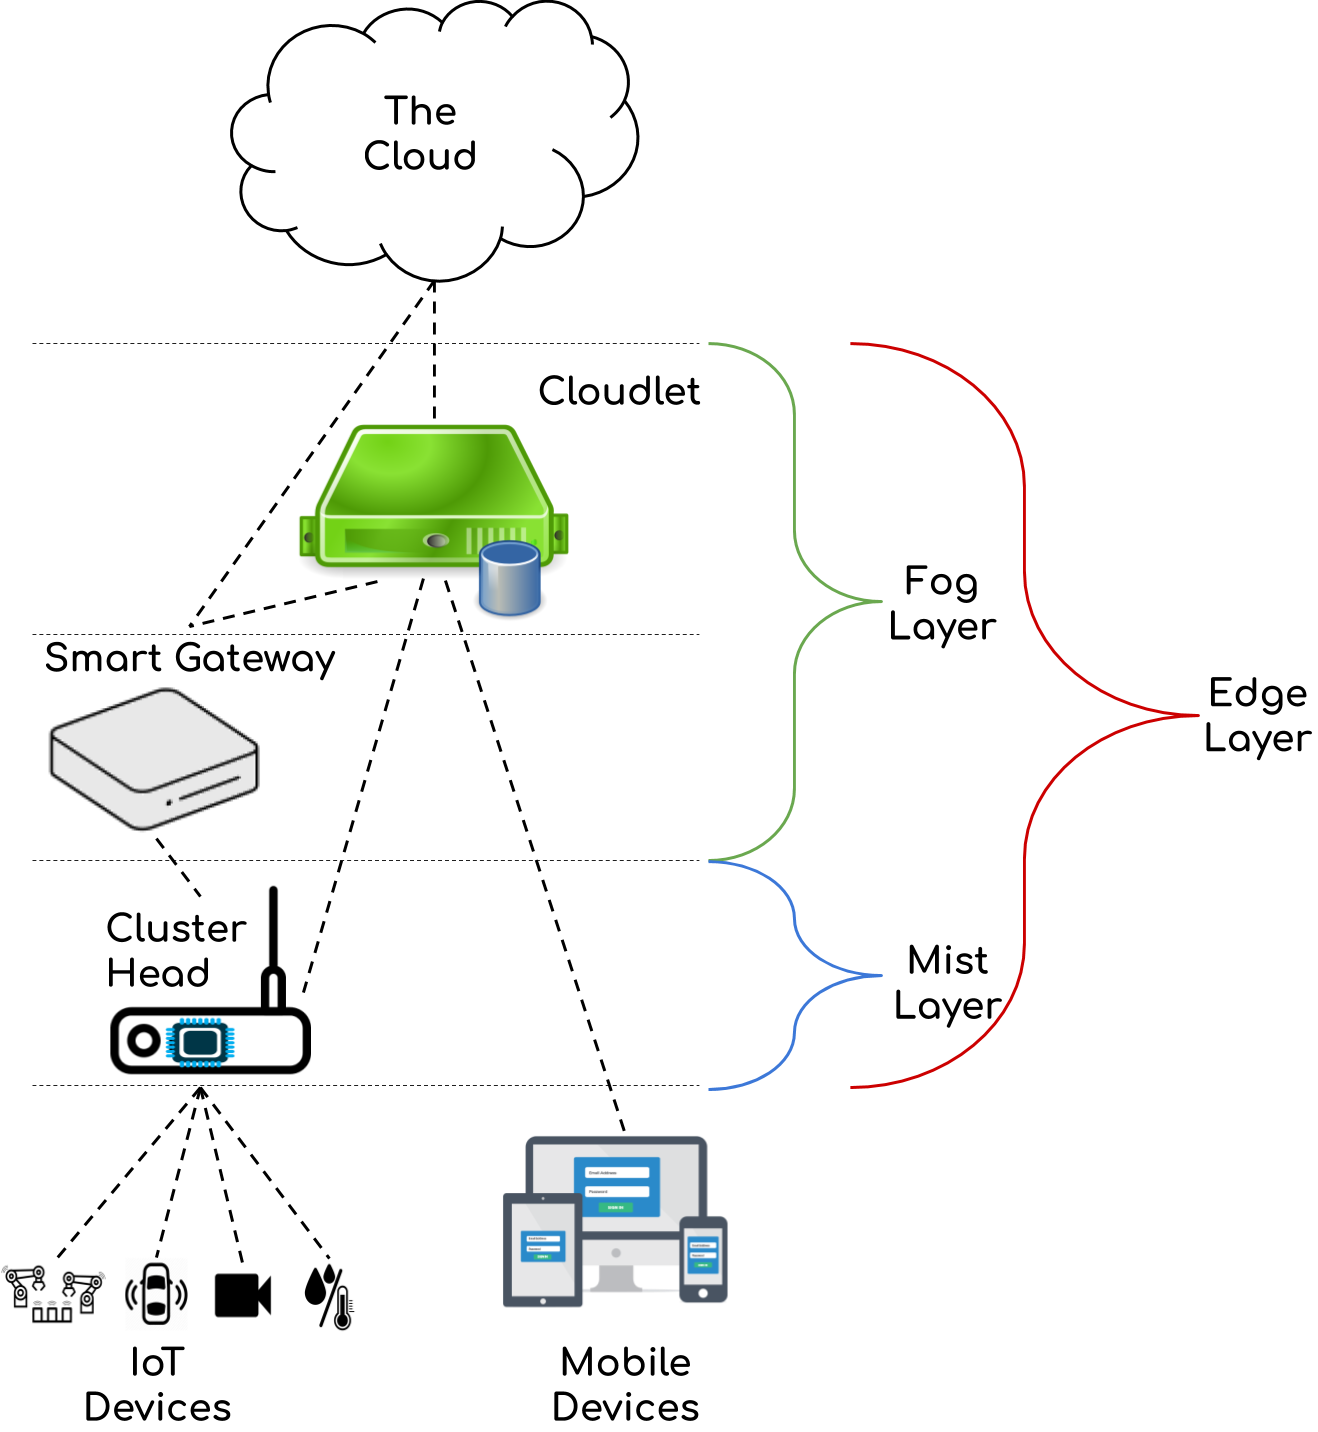
\includegraphics[scale=0.2]{figures/network-topology-3-layer.png}
    \mycaption[The Three Tier Layer Network Topology.]{It is similar to \cite{nsa2017NextWaveIoTDef}.}
    \label{fig:networkTopology3Layer}
\end{figure}

The cloud is well defined and understood. It describes the readily available computing resources over the Internet not managed by the user. The other layers and devices are not so well understood and defined separately.\\[5mm]
\textbf{\textit{Constrained Device}}\\
Constraint devices are an elementary part of the IoT making up the "things"\cite{contstraintDevicesTerminology}.
They can have three main purposes. Either sensing or actuating (or both), where sensing is the 
passive action of measuring the environment (e.g. a motion detector) and actuating is the active action of influencing the environment (e.g. control of pressure in test tube). Or, finally, they can be smart objects enhancing the interaction between other smart objects and people.
They are usually defined by their limitation, mainly, small computing power (CPU, RAM, storage etc.) and limited power supply and operate in constrained network using protocols like BLE and ZigBee. \\[5mm]
\textbf{\textit{Smart/mobile devices}}\\
Smart devices are not clearly defined in the academic literature. I will use the definition given by \citeauthor{poslad2011smartDevices}\cite{poslad2011smartDevices}, to clearly divide them from constrained devices which this thesis will be concerned with. They are traditional computing devices and "tend to be multi purpose ICT devices"\cite{poslad2011smartDevices}, examples are mobile phones (smart phones) or tablets. They connect to the rest of the infrastructure directly but are free to move between networks. They also often rely on battery power and, importantly, are mainly end user devices. This has important privacy implication, a major factor for edge computing.\\[5mm]
\textbf{\textit{IoT Cluster Head}}\\
IoT Cluster Heads are defined by their very limited processing power. They are used to combine multiple sensors or actuators, but do not perform powerful operations. The line between IoT Cluster Heads and IoT Gateways is constantly moving as devices get more powerful and software more efficient. In this paper, IoT Cluster Heads are defined as devices which are used to read and control IoT devices but are not powerful enough to run containers or Kubernetes.
\textbf{\textit{IoT Gateway}}\\
IoT gateways are the connection between constrained devices and the cloud. I will use the term IoT gateway and not only gateway to stress its relation with IoT. They are usually connected to a network, either local or the the Internet. They facilitate inter-network and intra-network communications and because smart devices and especially constrained devices often communicate via wireless and non-Internet protocols, IoT gateways often translate protocols "between wireless sensor networks [...] and traditional communication networks"\cite{zhu2010iotGatewayDefinition}.
In recent years IoT Gateways have become a major field of interest and new research. As these devices got more powerful, developers started using them for pre-processing and data gathering locally at the edge.
IoT gateways can take a wide variety of forms. They can be simple L2/L3 routers or more powerful devices. Importantly, they are situated at the edge of a network.\\[5mm]
\textbf{\textit{Edge Layer}}\\
The edge layer is a term used to describe all resources sitting at the edge of the network. They do not interact with their environment directly only through IoT or mobile devices. This line started to fade, when mobile devices where used to control IoT devices directly. In this research I will stick to definition that edge layer devices are no user facing devices.\\[5mm]
\textbf{\textit{Fog Layer}}\\
The fog layer and consequently fog computing is a term used to describe the logical extension of traditionally cloud resources to the edge. These devices are still connected to the overall system and are an active part in the data processing pipeline. Fog computing enables repeatable structure on the edge for better and more scalable performance.
\textbf{\textit{Mist Layer}}\\
The mist layer is not logically connected to the cloud and both are not part of the same system and function independently of each other. It can be that the cloud can indirectly control the mist layer through the fog devices but importantly the mist layer does not do tasks which were traditional done in the cloud. \\[5mm]
\textbf{\textit{Edge cluster}}\\
Edge clusters are two or more edge devices working together where one device needs to be powerful enough to run a full control plane of the cluster technology. With emerging technologies like tiny builds of a full Kubernetes cluster, e.g. K3s from Rancher Labs\cite{k3sLight14:online}, this is becoming increasingly easier and more popular.
\footnote{Rancher provides a 40MB Kubernetes binary and claims that 500MB of RAM is sufficient 
it stable.}.\\
\textbf{\textit{Edge node}}\\
Edge nodes are defined as nodes "that act as an end user portal for communication with other
nodes in cluster computing"\cite{Whatised17:edgeNodeDef}. The other nodes can either be edge nodes as well or cloud nodes. Importantly, edge nodes do not need to be able to run their own control plane.